% Chapter 3 from the thesis template file
%   that contains an example table and figure.
\chapter{METHODS AND PROCEDURES}

This is the opening paragraph to my thesis which
explains in general terms the concepts and hypothesis
which will be used in my thesis.

With more general information given here than really
necessary.

\section{Introduction}

Here initial concepts and conditions are explained and
several hypothesis are mentioned in brief.

As can be seen in Table~\ref{nothing} it is truly
obvious what I am saying is true.

\begin{table}[h!tb] \centering

\isucaption[Short caption for List of Figures/ Tables]{This table shows a standard empty table\autocite{kleeHellyTheoremIts1963} . Remove the square bracketed information to get longer captions in the LOT/ LOF }
\label{nothing}

\vspace{ 2 in}
\end{table}

\subsection{Hypothesis}

Here one particular hypothesis is explained in depth
and is examined in the light of current literature.

This can also be seen in Figure~\ref{moon} that the
rest is obvious.

\begin{figure}[h!tb] \centering

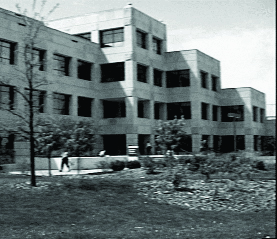
\includegraphics[alt={Alt text describing}]{Images/dc5.jpg}
\isucaption[Short caption for List of Figures/ Tables]{This table shows a standard empty figure. Remove the square bracketed information to get longer captions in the LOT/ LOF}
\label{moon}
\end{figure}

\subsubsection{Parts of the hypothesis}

Here one particular part of the hypothesis that is 
currently being explained is examined and particular
elements of that part are given careful scrutiny.

% Below \subsubsection
% Sectional commands: \paragraph and \subparagraph may also be used

\subsection{Second Hypothesis}

Here one particular hypothesis is explained in depth
and is examined in the light of current literature.

\subsubsection{Parts of the second hypothesis}

Here one particular part of the hypothesis that is 
currently being explained is examined and particular
elements of that part are given careful scrutiny.

%\addtocontents{toc}{\protect\newpage} % Adds \newpage in "\tableofcontents"
\section{Criteria Review}

Here certain criteria are explained thus eventually
leading to a foregone conclusion as can be seen in
Table~\ref{nevermore}.
%\tagpdfsetup{table/header-rows={1,2}} would have rows 1 and 2 be header rows
\tagpdfsetup{table/header-rows={1}}
%Use \tagpdfsetup{table/header-columns={}} for header columns instead
%Put \tagpdfsetup{table/multirow={⟨number of rows comma separated ⟩} in cells spanning multiple rows
\begin{table}[h!tb] \centering
    \begin{tabular}{c|c|c}
        Header & head  & head\\ 
        leg & leg & leg \\
        leg & leg & leg \\
        leg & leg & leg \\
    \end{tabular}
\setlength{\captionwidth}{3.5 in}
\isucaption{This table shows a standard empty table with
a limited captionwidth}
\label{nevermore}

\vspace{ 2 in}
\end{table}

